\documentclass[10pt,a4j,twocolumn]{jsarticle}

\usepackage[dvipdfmx]{graphicx}
\usepackage{listings}
\setlength{\textheight}{275mm}
\headheight 5mm
\topmargin -30mm
\textwidth 185mm
\oddsidemargin -15mm
\evensidemargin -15mm
\pagestyle{empty}
\begin{document}
\title{ユーザメモソフトmy\_helpのビヘイビアテスト開発}
\author{関西学院大学 情報科学科 西谷研究室 2535 那須比呂貴}
\date{}
\maketitle

\section{目的}
\vspace{-0.5em}
プログラム開発では,統合開発環境がいくつも用意されているが,多くの現場では,terminal上での開発が一般的である.ところが,プログラミング初心者はterminal上でのcharacter user interface(CUI)を苦手としている.この不可欠なCUIスキルの習得を助けるソフトとして,ユーザメモソフトmy\_helpがruby gemsに置かれている.しかし,Ruby gemsとして提供されているこのソフトは,テストが用意されていない.今後ソフトを共同開発を進めていくには,仕様や動作の標準となるテスト記述が不可欠である.本研究の目的は,ユーザメモソフトであるmy\_helpのテストをBDDを用いて開発することである.

\section{方法}
\vspace{-0.5em}
\paragraph{BDD}
ビヘイビア駆動開発(Behaviour-Driven Development : BDD)は,テスト駆動開発(Test-Driven Development : TDD)の工程への理解を深め,それをうまく説明しようとして始まった.TDDの持つ単語のイメージが構造のテストを中心とすべしというのに対して,BDDはソフトの振る舞いに中心をおくという意図がある.この違いが,初めに考えるべきテストの性質を変化させ,構造ではなく振る舞いを中心にテストを構築するという意識をもたせてくれる.さらに,実世界における開発チームやテストチーム,あるいはドキュメントチーム間のコミュニケーションの取り方を,システムで提供するのがBDDのフレームワークであり,CucumberとRSpecはこれを実現する一つのシステムとして提供されている\cite{RSpecBook}.

\paragraph{CucumberとRSpec}
図1はRSpecとCucumberの関係図である.BDDの流れとして,まずCucumberで一つのシナリオに焦点を当てて,その振る舞いを記述するfeatureを書く.一つのfeatureが書けたら、次に,それぞれfeatureを実現するステップに分けて仕様を決める.これはTDDのred green refactoringの前に行う作業,「仕様を決める」に対応している.このプロセスが終了したら,RSpecに進む.
RSpecでは実際にテストコードを書き,ここでもred, green, refactoringをおこない,RSpecが成功したら,Cucumberのrefactoringをおこなう.
\begin{figure}
\begin{center}
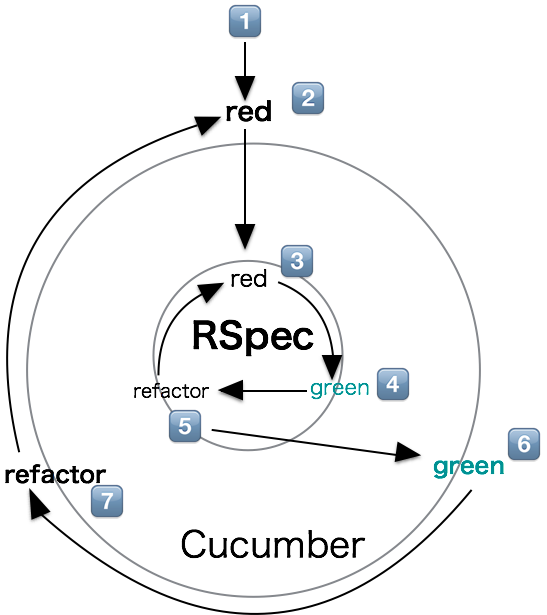
\includegraphics[width=5cm, bb=0 0 394 443]{abst_fig.png}
\caption{RSpecとCucumberのRed-Green-Refactoringサイクル間の関係.}
\end{center}
\vspace{-3em}
\end{figure}

\section{ビヘイビアテスト駆動開発の実践}
CucumberとRSpecを用いてBDDでmy\_helpのテスト開発を進めていった.
ここでは,焦点を合わせたmy\_helpの中での一つの振る舞いである「todoの更新」を例として詳しく見ていく.
\begin{description}
\item[cucumber]
\begin{enumerate}
\item まず,「todoの更新」のシナリオをfeatureで記述.
\item cucumberを実行するとステップの元なるコードブロックが自動生成されるので,それをコピー\&ペーストしてステップを記述.
\item ここではあれば良いなと思うコードを記述し,もう一度cucumberを実行.
\end{enumerate}
\item[rspec]
\item ここでは,エラーが出るはずで,そのシナリオに焦点をあて,RSpecに移行してテストコードを記述.
\item[cucumber] RSpecが成功したら,もう一度Cucumberに戻り,redをgreenに.
\end{description}
このようにして,BDDのコンセプトに従って,my\_helpの仕様や動作の標準を確定していった.

\section{まとめ}
\vspace{-0.5em}
my\_helpのテスト記述の進展に伴って,仕様や動作の標準が確定した.
my\_helpは今後も開発者,ならびに多くのユーザの使用を通じて,どのように進化させれば便利なのかが徐々にわかってくる.つまり,ビヘイビアの記述により,今後my\_helpを進化させるための共同開発が円滑に進める手助けになる.
さらに,my\_helpの使用方法が明確になったことで,本研究で作成したmy\_helpのfeaturesを読めば初心者でもmy\_helpの振る舞いが容易に理解できるようになった.

\begin{thebibliography}{99}
\bibitem{RSpecBook}   "The RSpec Book", David Chelimsky {\it et al.}, (翔泳社, 2012).
\end{thebibliography}
\end{document}